%% Created by Maple 2020.1, Linux
%% Source Worksheet: workshop_2.mw
%% Generated: Sun Dec 06 16:55:31 CET 2020
\documentclass{article}
\usepackage{amssymb}
\usepackage{graphicx}
\usepackage{hyperref}
\usepackage{listings}
\usepackage{maplestd2e}
\usepackage[utf8]{inputenc}
\begin{document}
\lstset{basicstyle=\ttfamily,breaklines=true,columns=flexible}
\pagestyle{empty}
\DefineParaStyle{Maple Bullet Item}
\DefineParaStyle{Maple Heading 1}
\DefineParaStyle{Maple Warning}
\DefineParaStyle{Maple Heading 4}
\DefineParaStyle{Maple Heading 2}
\DefineParaStyle{Maple Heading 3}
\DefineParaStyle{Maple Dash Item}
\DefineParaStyle{Maple Error}
\DefineParaStyle{Maple Title}
\DefineParaStyle{Maple Text Output}
\DefineParaStyle{Maple Normal}
\DefineCharStyle{Maple 2D Output}
\DefineCharStyle{Maple 2D Input}
\DefineCharStyle{Maple Maple Input}
\DefineCharStyle{Maple 2D Math}
\DefineCharStyle{Maple Hyperlink}
\begin{Maple Normal}{
\mapleinline{inert}{2d}{}{\[\]}
}\end{Maple Normal}
\section{\textbf{Workshop 2 - Kompleksitet af algoritmer}}
\begin{Maple Normal}{
En søgefunktion tager som input en liste (et array) af elementer (\mapleinline{inert}{2d}{a__1, a__2, () .. a__n}{$\displaystyle a_{1},\,a_{2},\,{\ldots a_{n}}$}
)\linebreak
sammen med et andet input x, som er det vi søger efter. Vi vil undersøge,\linebreak
om x er en del af vores liste, altså om \mapleinline{inert}{2d}{x = a__i}{$\displaystyle x=a_{i}$}
 for et i mellem 1 og n. Hvis\linebreak
\mapleinline{inert}{2d}{x = a__i}{$\displaystyle x=a_{i}$}
 vil vi returnere placeringen, altså i. Hvis x ikke er at finde i listen, så\linebreak
returnerer vi 0. Vi lader A være mængden af alle lister indeholdende heltal.\linebreak
Da kan vi betragte følgende:\linebreak
}\end{Maple Normal}

\begin{Maple Normal}{
\mapleinline{inert}{2d}{Typesetting:-mrow(Typesetting:-mi("f", italic = "true", mathvariant = "italic"), Typesetting:-mo(":", mathvariant = "normal", fence = "false", separator = "false", stretchy = "false", symmetric = "false", largeop = "false", movablelimits = "false", accent = "false", lspace = "0.2777778em", rspace = "0.2777778em"), Typesetting:-mi("A", italic = "true", mathvariant = "italic"), Typesetting:-mo(" ", mathvariant = "normal", fence = "false", separator = "false", stretchy = "false", symmetric = "false", largeop = "false", movablelimits = "false", accent = "false", lspace = "0.0em", rspace = "0.0em"), Typesetting:-mi("x", italic = "true", mathvariant = "italic"), Typesetting:-mo(" ", mathvariant = "normal", fence = "false", separator = "false", stretchy = "false", symmetric = "false", largeop = "false", movablelimits = "false", accent = "false", lspace = "0.0em", rspace = "0.0em"), Typesetting:-mi("&integers;", italic = "false", mathvariant = "normal"), Typesetting:-mo("&srarr;", mathvariant = "normal", fence = "false", separator = "false", stretchy = "false", symmetric = "false", largeop = "false", movablelimits = "false", accent = "false", lspace = "0.0em", rspace = "0.0em"), Typesetting:-mi("&naturals;", italic = "false", mathvariant = "normal"))}{\[f :A \mathop{\rm  }x \mathop{\rm  }\mathbb{Z}\rightarrow \mathbb{N}\]}
}\end{Maple Normal}
\begin{Maple Normal}{
\mapleinline{inert}{2d}{f(a__1, a__2, () .. a__n, x) = piecewise(x = a__i, i, x <> a__i, 0)}{\[f \left( a_{1},a_{2},{\ldots a_{n}},x \right) =\begin{cases}i & x=a_{i}\\0 & x\neq a_{i}\end{cases}\]}
}\end{Maple Normal}
\begin{Maple Normal}{
}\end{Maple Normal}
\subsection{\textbf{1.0}}
\begin{Maple Normal}{
\mapleinline{inert}{2d}{}{\[\]}
}\end{Maple Normal}
\subsubsection{\textbf{\textit{1.1}}}
\begin{Maple Normal}{
 Forklar hvorfor eksempelvis listen (3, 4, 4, 5) medfører, at f reelt set\linebreak
ikke er en funktion i matematisk forstand.\linebreak
}\end{Maple Normal}

\begin{Maple Normal}{
Saetter man \mapleinline{inert}{2d}{x = 4}{$\displaystyle x=4$}
 bliver resultatet baade 2 otg 3 dette kan vi ikke have.}\end{Maple Normal}

\begin{Maple Normal}{
\raisebox{4.152777777777778in}{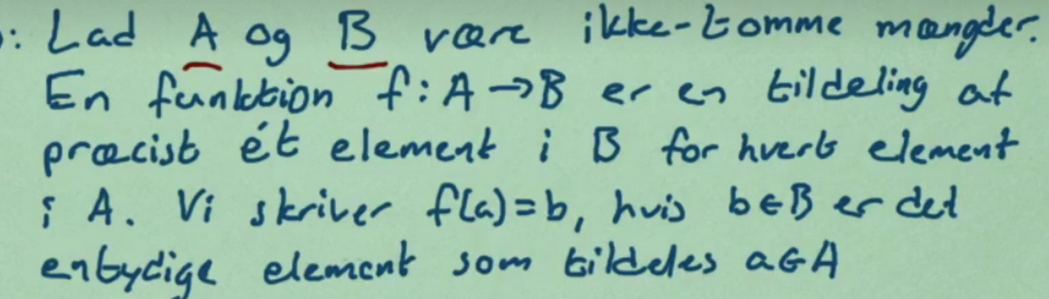
\includegraphics[keepaspectratio,height=4.152777777777778in]{workshop_2_image0.png}}}\end{Maple Normal}
\begin{Maple Normal}{
\mapleinline{inert}{2d}{}{\[\]}
}\end{Maple Normal}
\subsubsection{\textbf{\textit{1.2}}}
\begin{Maple Normal}{
Hvis vi i stedet definerer mængden A sådan, at lister i A ikke må\linebreak
indeholde det samme element to gange, så er f en funktion. Er f i\linebreak
dette tilfælde injektiv, surjektiv, bijektiv?\linebreak
\mapleinline{inert}{2d}{}{$\displaystyle $}
\raisebox{5.555555555555555in}{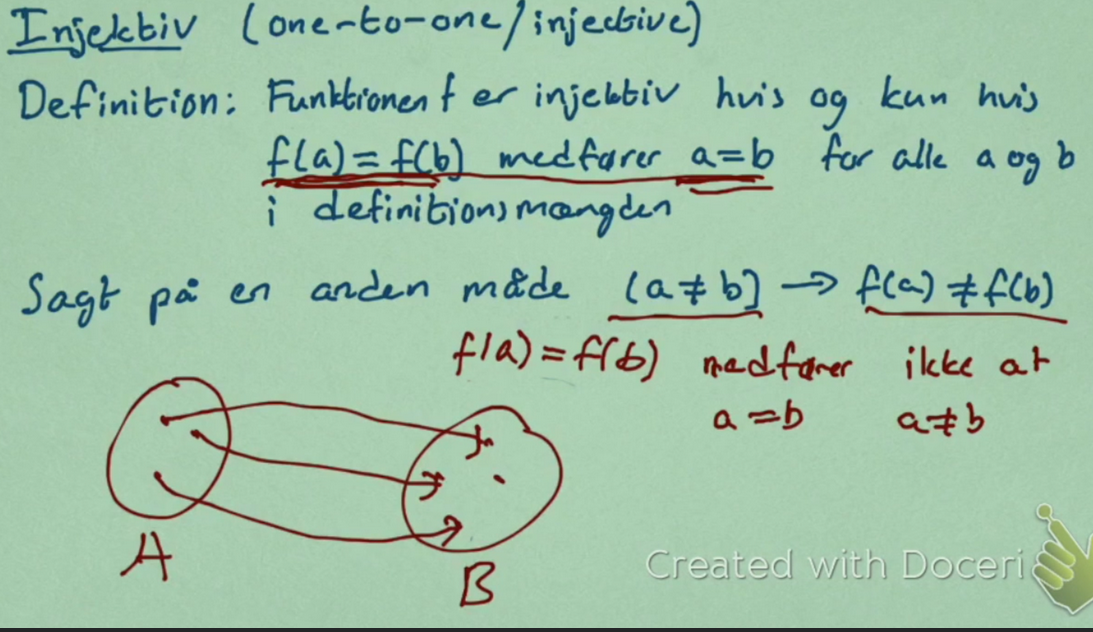
\includegraphics[keepaspectratio,scale=0.6329113924050633,height=5.555555555555555in]{workshop_2_image1.png}}}\end{Maple Normal}
\begin{Maple Normal}{
tag listerne:}\end{Maple Normal}

\begin{Maple Normal}{
[1, 3, 4] og [2, 3, 4] saa vil}\end{Maple Normal}

\begin{Maple Normal}{
\mapleinline{inert}{2d}{f([1, 3, 4], 2) = f([2, 3, 4], 2) and f([2, 3, 4], 2) = 2, [1, 3, 4] <> [2, 3, 4]}{\[f \left( [1,3,4],2 \right) =f \left( [2,3,4],2 \right)  \land f \left( [2,3,4],2 \right) =2,\,[1,3,4]\neq [2,3,4]\]}
}\end{Maple Normal}
\begin{Maple Normal}{
}\end{Maple Normal}
\begin{Maple Normal}{
\raisebox{5.708333333333333in}{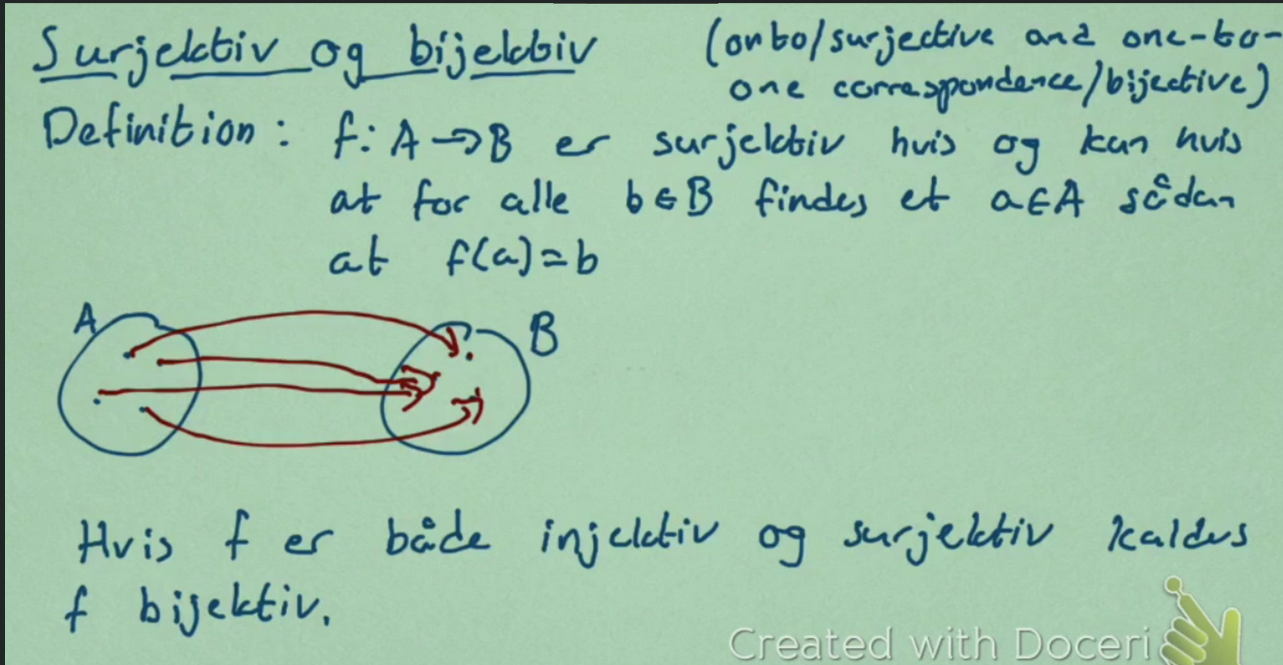
\includegraphics[keepaspectratio,scale=0.6180451127819548,height=5.708333333333333in]{workshop_2_image2.png}}}\end{Maple Normal}
\begin{Maple Normal}{
hvis A er alle lister med heltal vil man paa et eller andet tidspunkt faa}\end{Maple Normal}

\begin{Maple Normal}{
\mapleinline{inert}{2d}{f(N, 1) = 1}{\[f \left( N,1 \right) =1\]}
}\end{Maple Normal}
\begin{Maple Normal}{
\mapleinline{inert}{2d}{f(N, 2) = 2}{\[f \left( N,2 \right) =2\]}
}\end{Maple Normal}
\begin{Maple Normal}{
\mapleinline{inert}{2d}{() .. ()}{\[{\ldots }\]}
}\end{Maple Normal}
\begin{Maple Normal}{
\mapleinline{inert}{2d}{f(N, n) = n}{\[f \left( N,n \right) =n\]}
}\end{Maple Normal}
\begin{Maple Normal}{
}\end{Maple Normal}
\begin{Maple Normal}{
Da funktionen er surjektiv men ikke injektiv er den ikke bijektiv.\mapleinline{inert}{2d}{}{$\displaystyle $}
}\end{Maple Normal}

\subsection{\textbf{Pre 2.0 tekst}}
\begin{Maple Normal}{
På Figur 1 og 2 er to søgealgoritmer, som netop returnerer i hvis \mapleinline{inert}{2d}{x = a__i}{$\displaystyle x=a_{i}$}
 og\linebreak
0 ellers. Bemærk, at BinSearch kræver at listen er ordnet.}\end{Maple Normal}

\subsection{\textbf{2.0}}
\begin{Maple Normal}{
}\end{Maple Normal}
\subsubsection{\textbf{\textit{2.1}}}
\begin{Maple Normal}{
Implementer i SearchFunc.c de to søgealgoritmer fra Figur 1 og 2.1\linebreak
}\end{Maple Normal}

\begin{Maple Normal}{
\mapleinline{inert}{2d}{}{\[\]}
}\end{Maple Normal}
\subsubsection{\textbf{\textit{2.2}}}
\begin{Maple Normal}{
Undersøg om elementet 7000 er i listerne List500.txt, List1000.txt,\linebreak
List2000.txt, List4000.txt og List8000.txt. I den tilhørende kode køres\linebreak
begge algoritmer 1000000 gange og der tages tid på hvor lang tid hver\linebreak
algoritme bruger. Brug begge algoritmer og undersøg hvor lang tid det\linebreak
tager. Hvilken er hurtigst?\linebreak
binSearch}\end{Maple Normal}

\begin{Maple Normal}{
\mapleinline{inert}{2d}{}{$\displaystyle $}
\mapleinline{inert}{2d}{}{$\displaystyle $}
}\end{Maple Normal}
\subsubsection{\textbf{\textit{2.3}}}
\begin{Maple Normal}{
Skriv ned hvor lang tid algoritmerne bruger på de forskellige listestør-\linebreak
relser og plot det i et koordinatsystem (listestørrelsen ud af x-aksen og\linebreak
tiden af y-aksen).\linebreak
}\end{Maple Normal}

\begin{Maple Normal}{
\mapleinline{inert}{2d}{n := [500, 1000, 2000, 4000, 8000]; -1}{\[\]}
}\end{Maple Normal}
\begin{Maple Normal}{
\mapleinline{inert}{2d}{linTime := [2.224, 4.427, 8.847, 17.698, 35.363]; -1}{\[\]}
}\end{Maple Normal}
\begin{Maple Normal}{
\mapleinline{inert}{2d}{binTime := [0.59e-1, 0.67e-1, 0.75e-1, 0.75e-1, 0.89e-1]; -1}{\[\]}
}\end{Maple Normal}
\begin{Maple Normal}{
\mapleinline{inert}{2d}{with(plots); -1}{\[\]}
}\end{Maple Normal}
\begin{Maple Normal}{
\mapleinline{inert}{2d}{p1 := pointplot([n, linTime], color = "blue"); -1}{\[\]}
}\end{Maple Normal}
\begin{Maple Normal}{
\mapleinline{inert}{2d}{p2 := pointplot([n, binTime], color = "red"); -1}{\[\]}
}\end{Maple Normal}
\begin{Maple Normal}{
\mapleinline{inert}{2d}{display(p1, p2, labels = ["n", "tid"])}{\[{\it display} \left( {\it p1},{\it p2},{\it labels}=[``n''\\
\mbox{},``tid''] \right) \]}
}\end{Maple Normal}
\mapleresult
\mapleplot{workshop_2plot2d1.eps}
\begin{Maple Normal}{
\mapleinline{inert}{2d}{}{\[\]}
}\end{Maple Normal}
\begin{Maple Normal}{
\mapleinline{inert}{2d}{}{\[\]}
}\end{Maple Normal}
\subsubsection{\textbf{\textit{Psuedo kode}}}
\begin{Maple Normal}{
\mapleinline{inert}{2d}{}{$\displaystyle $}
\raisebox{5.763888888888889in}{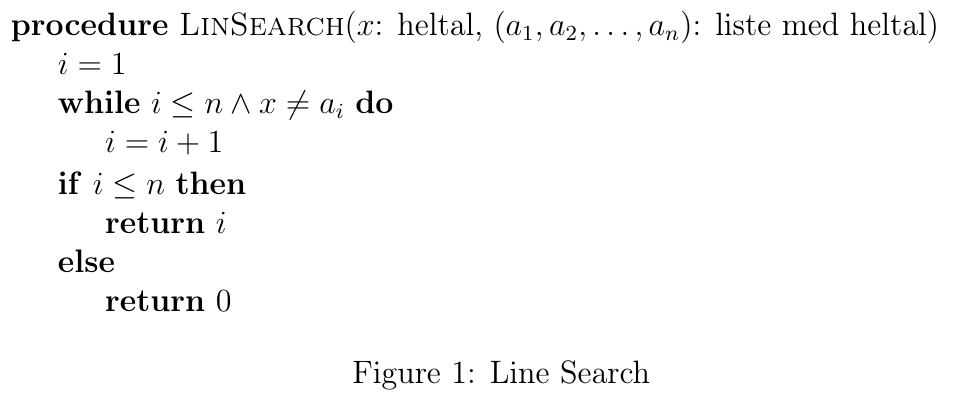
\includegraphics[keepaspectratio,height=5.763888888888889in]{workshop_2_image3.png}}}\end{Maple Normal}
\begin{Maple Normal}{
\raisebox{9.166666666666666in}{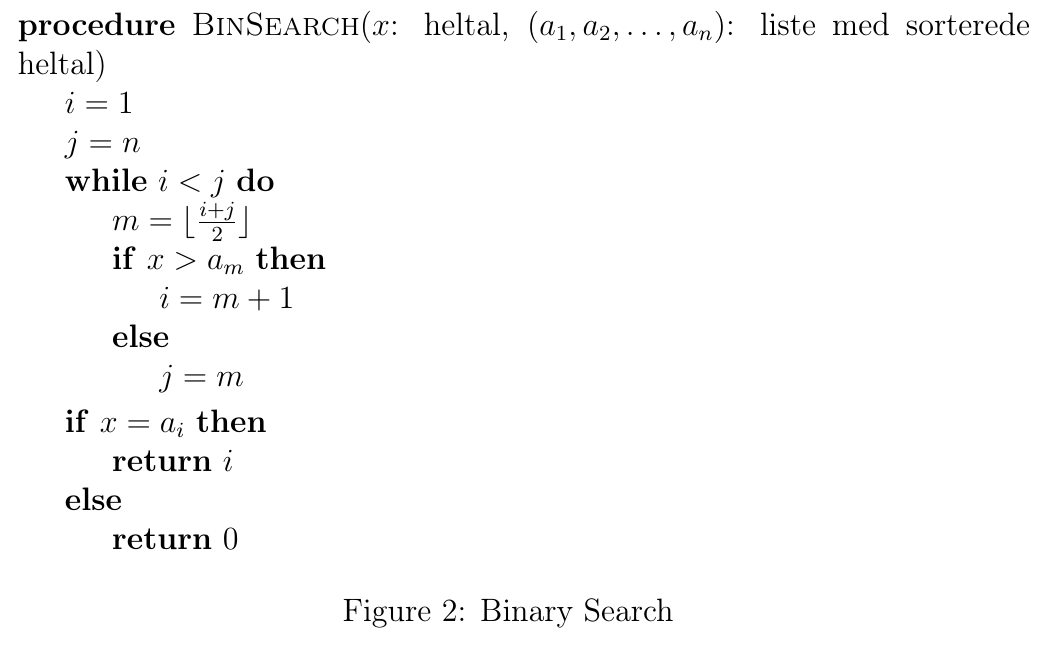
\includegraphics[keepaspectratio,height=9.166666666666666in]{workshop_2_image4.png}}\mapleinline{inert}{2d}{}{$\displaystyle $}
}\end{Maple Normal}
\begin{Maple Normal}{
}\end{Maple Normal}
\subsection{\textbf{Pre 3.0 tekst}}
\begin{Maple Normal}{
Vi kigger nu nærmere på den teoretiske kompleksitet for de to algoritmer.\linebreak
Her gennemgås worst-case tidskompleksiteten af BinSearch. For at holde\linebreak
det simpelt antager vi, at længden af listen er \mapleinline{inert}{2d}{n = 2^k}{$\displaystyle n={2}^{k}$}
 og tæller kun antallet\linebreak
af sammenligninger. Ved hvert gennemløb af while-løkken laves der 2 sam-\linebreak
menligninger. Spørgsmålet er så, hvor mange gennemløb af while-løkken vi\linebreak
har. Bemærk, at hvis \mapleinline{inert}{2d}{n = 2^k}{$\displaystyle n={2}^{k}$}
 bliver \mapleinline{inert}{2d}{m = 2^(k-1)}{$\displaystyle m={2}^{k-1}$}
 i første gennemløb. Derfor\linebreak
har vi reelt set halveret vores liste. Ved gennemløbene af while-løkken kigger\linebreak
vi derfor på lister af længde \mapleinline{inert}{2d}{2^k, 2^(k-1), 2^(k-2), () .. (), 2}{$\displaystyle {2}^{k},\,{2}^{k-1},\,{2}^{k-2},\,{\ldots },\,2$}
 og først når i = j er list-\linebreak
estørrelsen 1. Vi har derfor \mapleinline{inert}{2d}{k = log__2(n)}{$\displaystyle k={\it log}_{2} \left( n \right) $}
 gennemløb af while-løkken hvor der\linebreak
laves 2 sammenligninger for hver gennemløb. Læg dertil en sammenligning\linebreak
for while-løkken når i = j samt sammenligningen \mapleinline{inert}{2d}{x = a__i}{$\displaystyle x=a_{i}$}
 . Dette giver ialt\linebreak
\mapleinline{inert}{2d}{2*log__2(n)+2}{$\displaystyle 2\,{\it log}_{2} \left( n \right) +2$}
 sammenligninger.\linebreak
}\end{Maple Normal}

\subsection{\textbf{3.0}}
\begin{Maple Normal}{
\mapleinline{inert}{2d}{}{\[\]}
}\end{Maple Normal}
\subsubsection{\textbf{\textit{3.1}}}
\begin{Maple Normal}{
Læs og forstå udledningen af kompleksiteten for BinSearch.\linebreak
}\end{Maple Normal}

\begin{Maple Normal}{
\mapleinline{inert}{2d}{}{\[\]}
}\end{Maple Normal}
\subsubsection{\textbf{\textit{3.2}}}
\begin{Maple Normal}{
Forklar i hvilket tilfælde vi vil lave flest sammenligninger i LinSearch\linebreak
og at antallet af sammenligninger i dette tilfælde er 2n + 2.}\end{Maple Normal}

\begin{Maple Normal}{
\linebreak
I vaerste tilfaelde vil tallet vi leder efter ikke vaere i listen og algoritmen vil derfor gaa igennem hele listen}\end{Maple Normal}

\begin{Maple Normal}{
Man vil derfor gaa gennem while loekken n gange og man laver 2 sammenligninger hver gang altsaa 2n}\end{Maple Normal}

\begin{Maple Normal}{
naar i bliver stoerre end n laver vi endnu en sammenligning da i nu er stoerre end n sker der en short circuit }\end{Maple Normal}

\begin{Maple Normal}{
vi afslutter med at lave en sammenligning if vores if statement}\end{Maple Normal}

\begin{Maple Normal}{
altsaa faas 2n + 2}\end{Maple Normal}

\begin{Maple Normal}{
\mapleinline{inert}{2d}{}{\[\]}
}\end{Maple Normal}
\subsubsection{\textbf{\textit{3.3}}}
\begin{Maple Normal}{
Vis, at antallet af sammenligninger for LinSearch er \mapleinline{inert}{2d}{Theta(n)}{$\displaystyle \Theta \left( n \right) $}
, og at\linebreak
antallet af sammenligninger for BinSearch er \mapleinline{inert}{2d}{Theta(log(n))}{$\displaystyle \Theta \left( {\it log} \left( n \right)  \right) $}
 ved at finde\linebreak
vidner.}\end{Maple Normal}

\begin{Maple Normal}{
}\end{Maple Normal}
\begin{Maple Normal}{
Jeg gaar ud fra at de hentyder til log2 naar de skriver log\linebreak
}\end{Maple Normal}

\subsubsection{\textit{Store O}}
\begin{Maple Normal}{
}\end{Maple Normal}
\begin{Maple Normal}{
find (c, k) saa \mapleinline{inert}{2d}{abs(f(x)) <= C*abs(g(x))}{$\displaystyle  \left| f \left( x \right)  \right| \leq C \left| g \left( x \right)  \right| $}
 for alle x > k}\end{Maple Normal}

\begin{Maple Normal}{
}\end{Maple Normal}
\begin{Maple Normal}{
Lin}\end{Maple Normal}

\begin{Maple Normal}{
\mapleinline{inert}{2d}{abs(2*n+2) <= C*abs(n)}{\[ \left| 2\,n+2 \right| \leq C \left| n \right| \]}
}\end{Maple Normal}
\begin{Maple Normal}{
(4,1)}\end{Maple Normal}

\begin{Maple Normal}{
}\end{Maple Normal}
\begin{Maple Normal}{
Bin}\end{Maple Normal}

\begin{Maple Normal}{
\mapleinline{inert}{2d}{abs(2*log__2(x)+2) <= C*abs(log__2(x))}{\[ \left| 2\,{\it log}_{2} \left( x \right) +2 \right| \leq C \left| {\it log}_{2} \left( x \right)  \right| \]}
}\end{Maple Normal}
\begin{Maple Normal}{
x stoerre end 0}\end{Maple Normal}

\begin{Maple Normal}{
\mapleinline{inert}{2d}{2*log__2(x)+2 <= C*log__2(x)}{\[2\,{\it log}_{2} \left( x \right) +2\leq C{\it log}_{2} \left( x \right) \]}
}\end{Maple Normal}
\begin{Maple Normal}{
C=3}\end{Maple Normal}

\begin{Maple Normal}{
\mapleinline{inert}{2d}{2*log__2(x)+2 <= 3*log__2(x)}{\[2\,{\it log}_{2} \left( x \right) +2\leq 3\,{\it log}_{2} \left( x \right) \]}
}\end{Maple Normal}
\begin{Maple Normal}{
ved 4}\end{Maple Normal}

\begin{Maple Normal}{
(3, 4)}\end{Maple Normal}

\begin{Maple Normal}{
}\end{Maple Normal}
\subsubsection{\textit{Storo Omega}}
\begin{Maple Normal}{
find (c, k) saa \mapleinline{inert}{2d}{abs(f(x)) >= C*abs(g(x))}{$\displaystyle C \left| g \left( x \right)  \right| \leq  \left| f \left( x \right)  \right| $}
 for alle x > k}\end{Maple Normal}

\begin{Maple Normal}{
}\end{Maple Normal}
\begin{Maple Normal}{
Lin}\end{Maple Normal}

\begin{Maple Normal}{
\mapleinline{inert}{2d}{abs(2*n+2) >= C*abs(n)}{\[C \left| n \right| \leq  \left| 2\,n+2 \right| \]}
}\end{Maple Normal}
\begin{Maple Normal}{
(1,1)}\end{Maple Normal}

\begin{Maple Normal}{
}\end{Maple Normal}
\begin{Maple Normal}{
Bin}\end{Maple Normal}

\begin{Maple Normal}{
\mapleinline{inert}{2d}{abs(2*log__2(x)+2) >= C*abs(log__2(x))}{\[C \left| {\it log}_{2} \left( x \right)  \right| \leq  \left| 2\,{\it log}_{2} \left( x \right) +2 \right| \]}
}\end{Maple Normal}
\begin{Maple Normal}{
(1,1)}\end{Maple Normal}

\begin{Maple Normal}{
\mapleinline{inert}{2d}{}{\[\]}
}\end{Maple Normal}
\subsubsection{\textbf{\textit{3.4}}}
\begin{Maple Normal}{
 Sammenlign den teoretiske kompleksitet med det i fandt ud af i Delop-\linebreak
gave 2 (især koordinatsystemet).\linebreak
}\end{Maple Normal}

\begin{Maple Normal}{
\mapleinline{inert}{2d}{p3 := plot(x, x = 0 .. 8000); -1}{\[\]}
}\end{Maple Normal}
\begin{Maple Normal}{
\mapleinline{inert}{2d}{p4 := plot(log[2](x), x = 0 .. 8000); -1}{\[\]}
}\end{Maple Normal}
\begin{Maple Normal}{
\mapleinline{inert}{2d}{display(p1, p3)}{\[{\it display} \left( {\it p1},{\it p3} \right) \]}
}\end{Maple Normal}
\mapleresult
\mapleplot{workshop_2plot2d2.eps}
\begin{Maple Normal}{
\mapleinline{inert}{2d}{display(p2, p4)}{\[{\it display} \left( {\it p2},{\it p4} \right) \]}
}\end{Maple Normal}
\mapleresult
\mapleplot{workshop_2plot2d3.eps}
\begin{Maple Normal}{
\mapleinline{inert}{2d}{}{\[\]}
}\end{Maple Normal}
\begin{Maple Normal}{
\mapleinline{inert}{2d}{}{\[\]}
}\end{Maple Normal}
\subsubsection{\textbf{\textit{3.5}}}
\begin{Maple Normal}{
Det oplyses nu, at man kan sortere en liste ved at bruge \mapleinline{inert}{2d}{Theta(n*log(n))}{$\displaystyle \Theta \left( n{\it log} \left( n \right)  \right) $}
\linebreak
operationer. Vi får givet en usorteret liste med 10000 elementer og vi\linebreak
ved, at vi skal søge efter ca 50 elementer i listen. Giv ud fra store-Theta\linebreak
estimaterne (vi ser altså bort fra de oplyste konstanter i søgefunktion-\linebreak
erne) et bud på, om det bedst kan betale sig at sortere listen først\linebreak
og derefter bruge BinSearch eller om det er hurtigst at bruge Lin-\linebreak
Search.\linebreak
}\end{Maple Normal}

\begin{Maple Normal}{
\mapleinline{inert}{2d}{n := 10000; -1}{\[\]}
}\end{Maple Normal}
\begin{Maple Normal}{
\mapleinline{inert}{2d}{m := 50; -1}{\[\]}
}\end{Maple Normal}
\begin{Maple Normal}{
\mapleinline{inert}{2d}{res1 := n*log[2](n)+m*log[2](n)}{$\displaystyle {\it res1}\, := \,n{\it log}_{{2}} \left( n \right) +m{\it log}_{{2}} \left( n \right) $}
 = }\end{Maple Normal}

\mapleresult
\begin{maplelatex}
\mapleinline{inert}{2d}{40200*ln(10)/ln(2)}{\[40200\,{\frac {\ln  \left( 10 \right) }{\ln  \left( 2 \right) }}\]}
\end{maplelatex}
\begin{Maple Normal}{
\mapleinline{inert}{2d}{Typesetting:-mover(Typesetting:-mo("&rarr;", executable = "true", font_style_name = "2D Math", mathvariant = "normal", fence = "false", separator = "false", stretchy = "true", symmetric = "false", largeop = "false", movablelimits = "false", accent = "false", lspace = "0.2777778em", rspace = "0.2777778em"), Typesetting:-mtext("at 10 digits", executable = "true", font_style_name = "2D Math", mathvariant = "normal"), accent = "false")}{\[\Mapleoverset{}{\rightarrow }\]}
}\end{Maple Normal}
\mapleresult
\begin{maplelatex}
\mapleinline{inert}{2d}{133541.5094}{\[ 133541.5094\]}
\end{maplelatex}
\begin{Maple Normal}{
\mapleinline{inert}{2d}{res2 := m*n}{$\displaystyle {\it res2}\, := \,mn$}
 = }\end{Maple Normal}

\mapleresult
\begin{maplelatex}
\mapleinline{inert}{2d}{500000}{\[500000\]}
\end{maplelatex}
\begin{Maple Normal}{
\mapleinline{inert}{2d}{res1 < res2}{\[{\it res1}<{\it res2}\]}
}\end{Maple Normal}
\begin{Maple Normal}{
\mapleinline{inert}{2d}{Typesetting:-mover(Typesetting:-mo("&rarr;", executable = "true", font_style_name = "2D Math", mathvariant = "normal", fence = "false", separator = "false", stretchy = "true", symmetric = "false", largeop = "false", movablelimits = "false", accent = "false", lspace = "0.2777778em", rspace = "0.2777778em"), Typesetting:-mtext("test relation", executable = "true", font_style_name = "2D Math", mathvariant = "normal"), accent = "false")}{\[\Mapleoverset{}{\rightarrow }\]}
}\end{Maple Normal}
\mapleresult
\begin{maplelatex}
\mapleinline{inert}{2d}{true}{\[{\it true}\]}
\end{maplelatex}
\begin{Maple Normal}{
\mapleinline{inert}{2d}{}{\[\]}
}\end{Maple Normal}
\subsubsection{\textbf{\textit{3.6}}}
\begin{Maple Normal}{
Hvor mange søgninger skal man ca foretage for at de to tilgange er lige\linebreak
hurtige?}\end{Maple Normal}

\begin{Maple Normal}{
\linebreak
\mapleinline{inert}{2d}{m*n = n*log[2](n)+m*log[2](n)}{$\displaystyle mn=n{\it log}_{{2}} \left( n \right) +m{\it log}_{{2}} \left( n \right) $}
}\end{Maple Normal}

\begin{Maple Normal}{
\mapleinline{inert}{2d}{m*(n-log[2](n)) = n*log[2](n)}{\[m \left( n-{\it log}_{{2}} \left( n \right)  \right) =n{\it log}_{{2}} \left( n \right) \]}
}\end{Maple Normal}
\begin{Maple Normal}{
\mapleinline{inert}{2d}{m := n*log[2](n)/(n-log[2](n))}{$\displaystyle m\, := \,{\frac {n{\it log}_{{2}} \left( n \right) }{n-{\it log}_{{2}} \left( n \right) }}$}
 = }\end{Maple Normal}

\mapleresult
\begin{maplelatex}
\mapleinline{inert}{2d}{40000*ln(10)/((10000-4*ln(10)/ln(2))*ln(2))}{\[40000\,{\frac {\ln  \left( 10 \right) }{ \left( 10000-4\,{\frac {\ln  \left( 10 \right) }{\ln  \left( 2 \right) }} \right) \ln  \left( 2 \right) \\
\mbox{}}}\]}
\end{maplelatex}
\begin{Maple Normal}{
\mapleinline{inert}{2d}{Typesetting:-mover(Typesetting:-mo("&rarr;", executable = "true", font_style_name = "2D Math", mathvariant = "normal", fence = "false", separator = "false", stretchy = "true", symmetric = "false", largeop = "false", movablelimits = "false", accent = "false", lspace = "0.2777778em", rspace = "0.2777778em"), Typesetting:-mtext("at 10 digits", executable = "true", font_style_name = "2D Math", mathvariant = "normal"), accent = "false")}{\[\Mapleoverset{}{\rightarrow }\]}
}\end{Maple Normal}
\mapleresult
\begin{maplelatex}
\mapleinline{inert}{2d}{13.30539220}{\[ 13.30539220\]}
\end{maplelatex}
\begin{Maple Normal}{
}\end{Maple Normal}
\begin{Maple Normal}{
14}\end{Maple Normal}

\begin{Maple Normal}{
\mapleinline{inert}{2d}{solve(x*n = n*log[2](n)+x*log[2](n))}{$\displaystyle {\it solve} \left( xn=n{\it log}_{{2}} \left( n \right) +x{\it log}_{{2}} \left( n \right)  \right) $}
 = }\end{Maple Normal}

\mapleresult
\begin{maplelatex}
\mapleinline{inert}{2d}{-10000*ln(10)/(ln(10)-2500*ln(2))}{\[-10000\,{\frac {\ln  \left( 10 \right) }{\ln  \left( 10 \right) -2500\,\ln  \left( 2 \right) }}\]}
\end{maplelatex}
\begin{Maple Normal}{
\mapleinline{inert}{2d}{Typesetting:-mover(Typesetting:-mo("&rarr;", executable = "true", font_style_name = "2D Math", mathvariant = "normal", fence = "false", separator = "false", stretchy = "true", symmetric = "false", largeop = "false", movablelimits = "false", accent = "false", lspace = "0.2777778em", rspace = "0.2777778em"), Typesetting:-mtext("at 10 digits", executable = "true", font_style_name = "2D Math", mathvariant = "normal"), accent = "false")}{\[\Mapleoverset{}{\rightarrow }\]}
}\end{Maple Normal}
\mapleresult
\begin{maplelatex}
\mapleinline{inert}{2d}{13.30539220}{\[ 13.30539220\]}
\end{maplelatex}
\begin{Maple Normal}{
\mapleinline{inert}{2d}{}{\[\]}
}\end{Maple Normal}
\begin{Maple Normal}{
}\end{Maple Normal}
\begin{Maple Normal}{
\mapleinline{inert}{2d}{}{\[\]}
}\end{Maple Normal}
\end{document}
